\section{*应用：射影空间与透镜空间}
\sourcepage{287}
现在应用 CW 理论计算拓扑与几何中特别重要的射影空间的同调，并研究经典的三维流形——透镜空间。第 8.8、8.9 节计算这些空间的上同调环时将用到本节结果。

\entry{定义}{4.14.1}在 $S^n$ 上规定 $x\sim-x$，所得商空间称为\textbf{实 $n$ 维射影空间}（real projective $n$-space），记为 $P^n$。不致混淆时省略“实”。

商映射 $p:S^n\to P^n$ 是闭映射：若 $A\subset S^n$ 闭，其饱和集为 $A\cup a(A)$，其中 $a$ 是对径同胚，因此闭。由商拓扑定义，$p(A)$ 闭。所以 $P^n$ 为 Hausdorff 空间，事实上正规。

将 $\R^n$ 视为只有前 $n$ 项可非零的序列空间，则 $\R^n\subset\R^{n+1}$，相应有赤道包含 $S^{n-1}\subset S^n$。对径关系在两者上一致，故 $P^{n-1}\subset P^n$，且为闭子空间：$C\subset P^{n-1}$ 的原像在 $S^{n-1}$ 中闭，当且仅当在 $S^n$ 中闭，所以 $C$ 在这两个射影空间中的闭性一致。

\sourcepage{288}
\entry{定理}{4.14.2}$P^n$ 是零至 $n$ 维各有一个胞腔的 CW 复形，$j$ 维骨架为 $P^j$。

\textbf{证明：}$P^0$ 为一点。归纳地，把 $p$ 限制到闭上半球 $E^n_+$，得到连续满射 $p'$。定义域紧、值域 Hausdorff，故为商映射。它在开上半球上一一对应地映到 $P^n\setminus P^{n-1}$；此限制也是商映射，故为同胚，所得开 $n$ 维胞腔记为 $e_n$。边界 $S^{n-1}$ 映到低维骨架 $P^{n-1}$。将半球与 $B^n$ 认同，$p'$ 就是特征映射，归纳完成。\hfill$\square$

特别地，$P^1$ 是一条开边的两个端点粘到一点所得的圆周。

\entry{定义}{4.14.3}递增列 $P^0\subset P^1\subset\cdots$ 的协调并记为 $P^\infty$，称为\textbf{无限维实射影空间}。

现在将实数替换为复数。令 $\mathbb C^n$ 为第 $n$ 项以后为零的复数序列空间。\textbf{实化算子}（realification operator）
\[
\rho:\mathbb C^{n+1}\to\R^{2n+2},\qquad
\rho(z_1,z_2,\ldots)=(\operatorname{Re}z_1,\operatorname{Im}z_1,\operatorname{Re}z_2,\operatorname{Im}z_2,\ldots)
\]
是显然的同胚。定义 $|z|=\|\rho(z)\|=(\sum z_i\overline z_i)^{1/2}$。复序列中 $|z|=1$ 的子空间称为复 $n$ 维球面；它经实化对应 $S^{2n+1}$，因此无论在复空间还是实空间中，都用该记号。

\sourcepage{289}
\entry{定义}{4.14.4}在 $S^{2n+1}\subset\mathbb C^{n+1}$ 中，规定 $z\sim\lambda z$，其中 $|\lambda|=1$。所得商空间称为\textbf{复 $n$ 维射影空间}（complex projective $n$-space），记为 $\mathbb CP^n$。

商映射 $p$ 仍为闭映射：闭集 $A$ 的饱和集是紧集 $S^1\times A$ 经连续标量乘法 $(\lambda,z)\mapsto\lambda z$ 的像，故紧且闭。因此 $\mathbb CP^n$ 正规。由坐标包含，还得到闭子空间 $\mathbb CP^{n-1}\subset\mathbb CP^n$。一个等价类属于该子空间，当且仅当其任一代表满足 $z_{n+1}=0$。

\entry{定理}{4.14.5}$\mathbb CP^n$ 是 $2n$ 维 CW 复形，在每个偶数维 $0,2,\ldots,2n$ 恰有一个胞腔，$2j$ 维骨架为 $\mathbb CP^j$。

\textbf{证明：}$\mathbb CP^0$ 为一点。一般地，在单位复球面中要求 $z_{n+1}$ 为实数，所得集合经实化为 $S^{2n}$；再要求 $z_{n+1}\ge0$，得到其闭上半球 $E^{2n}_+$。限制映射 $p':E^{2n}_+\to\mathbb CP^n$ 是商映射，边界 $z_{n+1}=0$ 的像为 $\mathbb CP^{n-1}$。只需说明内部一一对应地映到 $e_{2n}=\mathbb CP^n\setminus\mathbb CP^{n-1}$，于是该限制为同胚，$p'$ 为特征映射。

满射性：对 $z_{n+1}\ne0$，写 $z_{n+1}=re^{i\theta}$，$r>0$。令 $\lambda=e^{-i\theta}$，则 $\lambda z$ 的末坐标为正实数 $r$，位于开半球中，且 $p(\lambda z)=p(z)$。

\sourcepage{290}
单射性：若开半球中的 $z,w$ 有同一像，则 $w=\lambda z$。末坐标均为正实数，迫使 $\lambda$ 为正实数；又 $|\lambda|=1$，故 $\lambda=1$，$w=z$。\hfill$\square$

特别地，$\mathbb CP^1$ 是把二维胞腔边界粘到一点所得空间，故同胚于 $S^2$。

\entry{定义}{4.14.6}递增列 $\mathbb CP^0\subset\mathbb CP^1\subset\cdots$ 的协调并称为\textbf{无限维复射影空间}，记为 $\mathbb CP^\infty$。由定理 4.12.15，它在每个非负偶数维各有一个胞腔，$2n$ 维骨架为 $\mathbb CP^n$。

\entry{定理}{4.14.7}$H_i(\mathbb CP^n)$ 在 $i$ 为偶数且 $0\le i\le2n$ 时为无限循环群，其余为零；$H_i(\mathbb CP^\infty)$ 在 $i$ 为非负偶数时为无限循环群，其余为零。

\textbf{证明：}胞腔链群仅在上述偶数维非零，且为无限循环群，因此所有边缘算子为零，每个链均闭，没有非零链是边缘。\hfill$\square$

实射影空间每一维都有胞腔，故必须详细计算边缘算子。由于 $e_k=P^k\setminus P^{k-1}$、$\dot e_k=P^{k-1}$，有 $D_k(P^n)=H_k(P^k,P^{k-1})$。我们需要计算相邻维之间的连接同态。

\entry{引理}{4.14.8}设 $n\ge1$，$p:S^n\to P^n$ 为商映射，$j:P^n\to(P^n,P^{n-1})$ 为包含映射。复合
\[
H_n(S^n)\xrightarrow{p_*}H_n(P^n)\xrightarrow{j_*}H_n(P^n,P^{n-1})
\]
在 $n$ 偶时为零，在 $n$ 奇时为乘以 $2$（选取适当生成元）。

\sourcepage{291}
\textbf{链层次的证明：}暂设球面与射影空间已三角剖分，使对径映射 $a$ 及投影 $p$ 都为单纯映射；引理 4.14.11 将证明可以做到。

取 $(E^n_+,S^{n-1})$ 的基本闭链 $c_n$。由引理 4.13.3，$p_\#c_n$ 是 $(P^n,P^{n-1})$ 的基本闭链。令 $\gamma_n=c_n+(-1)^{n-1}a_\#c_n$。因为赤道上的对径映射的度为 $(-1)^n$，它在顶维闭链群上为乘以此数，故
\[
\partial\gamma_n=\partial c_n+(-1)^{n-1}a_\#\partial c_n
=\partial c_n+(-1)^{2n-1}\partial c_n=0.
\]
此闭链在上半球的限制为基本闭链 $c_n$，所以不是其他闭链的非平凡倍数，因而是球面的基本闭链。由 $pa=p$，
\[
p_\#\gamma_n=[1+(-1)^{n-1}]p_\#c_n,
\]
即得结论。\hfill$\square$

\textbf{同调层次的证明：}下面在同调而非链上进行同样的计算。

\textbf{步骤 1。}考虑图中各包含映射 $i,k,\ell,m$ 及对径映射，取 $\alpha$ 为 $H_n(E^n_+,S^{n-1})$ 的生成元。
\begin{center}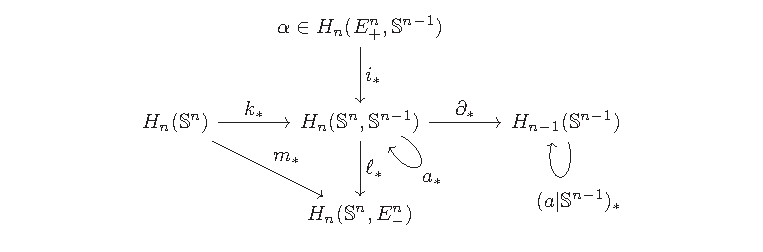
\includegraphics[width=.96\textwidth]{figures/4-14-diagram1.pdf}\end{center}
\sourcepage{292}
令 $\gamma=i_*\alpha+(-1)^{n-1}a_*i_*\alpha\in H_n(S^n,S^{n-1})$。\translatornote{原书把此处 $\gamma$ 所在群误印为 $H_n(E^n_+,S^{n-1})$。}由连接同态自然性及赤道对径映射的度，
\[
\partial_*\gamma=\partial_*i_*\alpha+(-1)^{n-1}(a|_{S^{n-1}})_*\partial_*i_*\alpha=0.
\]
由横向正合性，存在 $\beta\in H_n(S^n)$，使 $k_*\beta=\gamma$。

还需证明 $\beta$ 为生成元。由半球可缩，$m_*:H_n(S^n)\to H_n(S^n,E^n_-)$ 为同构，因此只需证明 $m_*\beta=\ell_*\gamma$ 生成。第一项 $\ell_*i_*\alpha$ 由定理 4.4.11 证明中的同构而生成该群；第二项 $\ell_*a_*i_*\alpha$ 为零，因为映射
\[
(E^n_+,S^{n-1})\xrightarrow{a}(E^n_-,S^{n-1})\longrightarrow(S^n,E^n_-)
\]
经过 $(E^n_-,E^n_-)$ 分解。因此 $\ell_*\gamma$ 确为生成元。

\textbf{步骤 2。}考虑下面的交换图，生成元按步骤 1 选择。
\begin{center}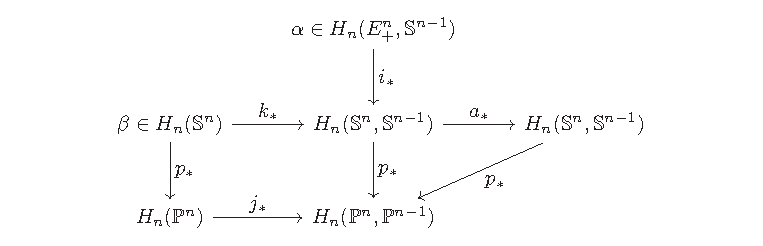
\includegraphics[width=.96\textwidth]{figures/4-14-diagram2.pdf}\end{center}
复合 $pi:(E^n_+,S^{n-1})\to(P^n,P^{n-1})$ 是胞腔特征映射，故 $p_*i_*\alpha$ 为生成元。于是
\[
j_*p_*\beta=p_*k_*\beta
=p_*(i_*\alpha+(-1)^{n-1}a_*i_*\alpha)
=[1+(-1)^{n-1}]p_*i_*\alpha,
\]
其中用了 $pa=p$，结论成立。\hfill$\square$

\sourcepage{293}
\entry{定理}{4.14.9}胞腔边缘 $H_{n+1}(P^{n+1},P^n)\to H_n(P^n,P^{n-1})$ 在 $n$ 偶时为零，在 $n$ 奇时将生成元映为生成元的两倍。

\textbf{证明：}特征映射 $p':(E^{n+1}_+,S^n)\to(P^{n+1},P^n)$ 诱导同构。上半球可缩，连接同态 $H_{n+1}(E^{n+1}_+,S^n)\to\widetilde H_n(S^n)$ 为同构。由连接同态自然性，所求胞腔边缘与上一引理中的 $j_*p_*$ 对应，故得结论。\translatornote{零维处应使用约化同调，才能使这里的连接同态为同构；原书图中统一写成了普通同调。}\hfill$\square$

\entry{定理}{4.14.10}实射影空间的约化同调为
\[
\widetilde H_i(P^{2n+1})\cong\begin{cases}\Z/2,&i\text{ 奇且 }0<i<2n+1,\\\Z,&i=2n+1,\\0,&\text{其他},\end{cases}
\]
\[
\widetilde H_i(P^{2n})\cong\begin{cases}\Z/2,&i\text{ 奇且 }0<i<2n,\\0,&\text{其他},\end{cases}\qquad
\widetilde H_i(P^\infty)\cong\begin{cases}\Z/2,&i>0\text{ 奇},\\0,&\text{其他}.\end{cases}
\]
\textbf{证明：}无限维射影空间的增广胞腔链复形各非负维均为 $\Z$，偶数正维的边缘为乘以 $2$，奇数维边缘为零，增广为恒等同态：
\[
\cdots\xrightarrow{0}\Z\xrightarrow{2}\Z\xrightarrow{0}\Z\xrightarrow{2}\Z\xrightarrow{0}\Z\xrightarrow{1}\Z.
\]
正偶数维没有非零闭链，正奇数维每个链均闭，而边缘恰为生成元的偶数倍。因此约化同调如述。有限维情形只需截断该链复形，即得相应结果。\hfill$\square$

\sourcepage{294}
\entry{引理}{4.14.11}可对 $S^n,P^n$ 三角剖分，使对径映射 $a$ 与商映射 $p$ 都为单纯映射。

\textbf{证明：步骤 1。}先归纳构造复形 $L\subset\R^{n+1}$ 及三角剖分 $k:|L|\to S^n$，使每个坐标反射 $\rho_i$ 都诱导 $L$ 的线性自同构，并与 $k$ 可交换。零维显然。若 $h:|K|\to S^{n-1}$ 已满足要求，取南北极 $w_0,w_1$，令 $L=(w_0*K)\cup(w_1*K)$。定义
\[
k((1-t)x+tw_0)=(\sqrt{1-t^2}\,h(x),t),\quad
k((1-t)x+tw_1)=(\sqrt{1-t^2}\,h(x),-t).
\]
它与所有坐标反射可交换，正是定理 2.9.8 中使用的三角剖分。

\textbf{步骤 2。}对径映射与 $k$ 可交换，并在 $L$ 及其每次重心重分上诱导线性自同构。取重分次数 $N$ 足够大，使每个顶点 $v$ 与 $a(v)$ 的闭星不交。用第 1.4 节的顶点标号方法，给每对 $v,a(v)$ 同一标号，构造商复形 $M$。所得单纯商映射只认同 $x$ 与 $a(x)$，不作其他认同。由于 $k$ 与对径映射可交换，它诱导 $|M|\to P^n$ 的同胚，得到所求三角剖分。\hfill$\square$

下面定义一类三维流形——透镜空间，并计算其同调。它们是少数已完全按同胚类型和同伦类型分类的空间族之一，分类问题稍后讨论。

\sourcepage{295}
\entry{定义}{4.14.12}设 $n,k$ 为互素正整数。把 $B^3$ 中的点写为 $(z,t)$，其中 $z$ 为复数、$t$ 为实数，$|z|^2+t^2\le1$。令 $\lambda=e^{2\pi i/n}$，定义球面上的映射
\[
f(z,t)=(\lambda^kz,-t).
\]
把下半球中每点 $x$ 与上半球中的 $f(x)$ 认同，所得商空间称为\textbf{透镜空间}（lens space），记为 $L(n,k)$。映射 $f$ 先绕竖直轴旋转 $2\pi k/n$，再关于水平面反射。
\begin{center}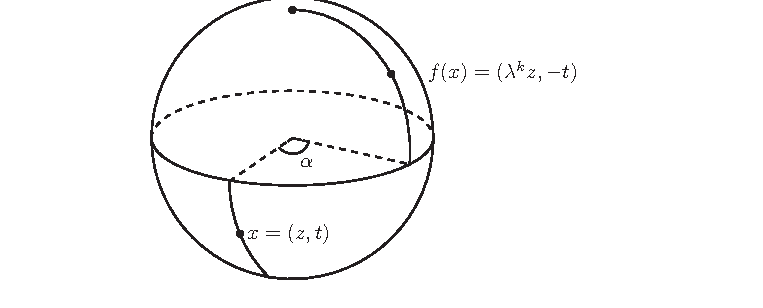
\includegraphics[width=.96\textwidth]{figures/4-14-1.pdf}\\图 4.14.1\end{center}
商映射 $p:B^3\to L(n,k)$ 在球内部不作认同，在两个开半球间成对认同。赤道点 $(z,0)$ 的等价类则为
\[
\{(\lambda^{jk}z,0):j=0,1,\ldots,n-1\}.
\]
因为 $k,n$ 互素，它与 $\{(\lambda^jz,0):0\le j<n\}$ 相同，恰为赤道上均匀分布的 $n$ 点。\translatornote{原书列举这些点时，若干项漏印了因子 $z$；此处用集合公式统一表达。}

\entry{定理}{4.14.13}$L(n,k)$ 是零、一、二、三维各有一个胞腔的 CW 复形。

\sourcepage{296}
\textbf{证明：}先证商映射闭。若 $A\subset B^3$ 闭，其饱和集是下列有限个紧集之并：
\[
A,\quad f(E^2_-\cap A),\quad f^{-1}(E^2_+\cap A),\quad
f^j(A\cap S^1)\ (1\le j<n).
\]
因此饱和集闭，$p(A)$ 闭，商空间正规且 Hausdorff。

取赤道点 $a=(1,0)$，以 $p(a)$ 为零维胞腔。令 $A$ 为从 $a$ 到 $b=(\lambda,0)$ 沿正方向的一段基本弧。限制 $p|_A$ 认同两端，内部则一一对应，所以 $p(\Int A)$ 为一维开胞腔，其特征映射为 $p|_A$。赤道由 $n$ 段这样的基本弧组成，每段内部都同胚地映到同一开胞腔。
\begin{center}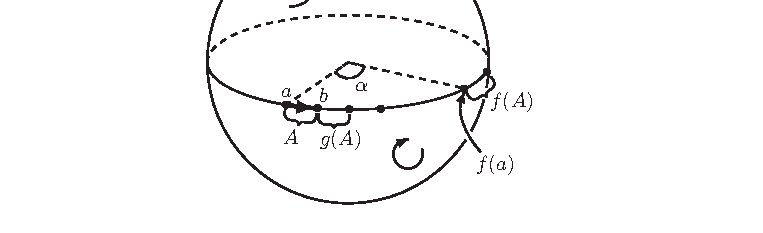
\includegraphics[width=.96\textwidth]{figures/4-14-2.pdf}\\图 4.14.2\end{center}
类似地，$p|_{E^2_-}$ 为二维胞腔的特征映射，内部像为开胞腔；整个 $p$ 为三维胞腔的特征映射，球内部的像为开胞腔。赤道像是一维骨架，球面像是二维骨架。\translatornote{原书称 $A$ 为“两点间的较小弧”。当 $n=1$ 时两端相同，需以完整圆周的一次参数化替代基本弧；可先把球赤道选一点和一条开边，再作同样的胞腔粘合。}\hfill$\square$

\sourcepage{297}
\entry{定理}{4.14.14}若 $X=L(n,k)$，则胞腔链复形为
\[
D_3(X)\xrightarrow{0}D_2(X)\xrightarrow{n}D_1(X)\xrightarrow{0}D_0(X),
\]
每个链群均为无限循环群。因此
\[
H_3(X)\cong\Z,\qquad H_2(X)=0,\qquad H_1(X)\cong\Z/n,\qquad H_0(X)\cong\Z.
\]
所以 $L(n,k)$ 与 $L(m,\ell)$ 若同胚，甚至若仅同伦等价，也必须有 $n=m$。

\textbf{证明：}可对 $B^3,L(n,k)$ 三角剖分，使旋转反射 $f$ 及商映射 $p$ 单纯；证明留作习题。

取基本闭链 $c_1$ 生成 $H_1(A,\Bd A)$，$c_2$ 生成 $H_2(E^2_-,S^1)$，$c_3$ 生成 $H_3(B^3,S^2)$。其像分别生成三个正维胞腔链群。先选 $c_1$ 的符号，使 $\partial c_1=b-a$。令
\[
z_1=c_1+f_\#c_1+\cdots+f_\#^{n-1}c_1.\tag{*}
\]
下面证明它生成 $H_1(S^1)$，然后选择 $c_2$ 的符号使 $\partial c_2=z_1$；再证明
\[
z_2=c_2-f_\#c_2\tag{**}
\]
生成 $H_2(S^2)$，据此选 $c_3$ 使 $\partial c_3=z_2$。

令 $g(z,0)=(\lambda z,0)$。因为赤道上 $f=g^k$，且 $k,n$ 互素，$f$ 的各次迭代将基本弧排列为与 $g$ 各次迭代相同的全部弧。因此
\[
z_1=c_1+g_\#c_1+\cdots+g_\#^{n-1}c_1.
\]
\translatornote{原书称赤道上 $g$ 与 $f$ 相同，这只在 $k\equiv1\pmod n$ 时成立。这里使用的是两者迭代项组成同一集合，因此求和相等。}由 $\partial c_1=g_\#a-a$，得
\[
\partial z_1=\sum_{j=0}^{n-1}(g_\#^{j+1}a-g_\#^ja)=0.
\]
它在基本弧上的限制为 $c_1$，所以是圆周的基本闭链，确为生成元。

再由 (*)，$f_\#z_1=z_1$，故 $\partial z_2=z_1-f_\#z_1=0$。其在下半球上的限制是基本闭链 $c_2$，因此它是球面的基本闭链。这样就能按计划选择 $c_2,c_3$ 的符号。

\sourcepage{298}
现在计算边缘。首先，$\partial p_\#c_1=p_\#b-p_\#a=0$。其次，因为赤道上 $pf^j=p$，
\[
\partial p_\#c_2=p_\#z_1=np_\#c_1.
\]
最后，因为下半球上 $pf=p$，
\[
\partial p_\#c_3=p_\#z_2=p_\#(c_2-f_\#c_2)=0.
\]
这给出所述链复形与同调群。\hfill$\square$

\entry{定理}{4.14.15}若 $k\equiv\pm\ell\pmod n$ 或 $k\ell\equiv\pm1\pmod n$，则透镜空间 $L(n,k)$ 与 $L(n,\ell)$ 同胚。习题 4 将引导证明。

\entry{注}{4.14.16}其逆命题也成立，但证明很困难。Kurt Reidemeister 在 1935 年的论文 [Rei35] 中定义了单纯复形的\textbf{挠率}（torsion），它是组合不变量：有同构重分的复形具有相同挠率。计算透镜空间挠率后，他证明若两个透镜空间的复形有同构重分，则必须满足上述同余条件。

要由此完成同胚分类，还需 E. E. Moise 在二十世纪五十年代关于三维流形仿射结构的研究。其系列论文第五篇 [Moi52] 证明：两个同胚的三角剖分三维流形必有同构的重分。因此透镜空间的同胚分类已知；第 8.9 节将讨论同伦类型分类。

\sourcepage{299--300}
\subsection*{习题}
\begin{enumerate}
\item 证明 $P^n$ 同胚于在 $B^n$ 的边界上认同 $x$ 与 $-x$ 所得商空间。\translatornote{原书把球误印为 $B^3$；按边界 $S^{n-1}$ 及一般维数，应为 $B^n$。}
\item \begin{enumerate}[label=(\alph*)]
\item 证明 $P^n$ 是 $n$ 维流形，$\mathbb CP^n$ 是 $2n$ 维流形。
\item 更一般地，证明有限维齐性 CW 复形是流形。
\end{enumerate}
\item 设 $A$ 为正 $n$ 边形围成的平面闭区域，$B$ 为它的悬挂。将 $L(n,k)$ 描述为 $B$ 的商空间，并推出可三角剖分 $B^3$ 与 $L(n,k)$，使商映射单纯。
\item 按下列步骤证明定理 4.14.15。
\begin{enumerate}[label=(\alph*)]
\item 考虑 $B^3$ 中反射 $(z,t)\mapsto(z,-t)$，证明 $k\equiv\pm\ell\pmod n$ 的情形。
\item 为方便设 $1\le k<n$。取以 $\Z/n$ 为指标的 $n$ 个不交三维单形 $a_ib_ic_id_i$，见图 4.14.3。证明 $L(n,k)$ 可按下列两步得到：先逐一将面 $a_ib_id_i$ 与 $a_{i+1}b_{i+1}c_{i+1}$ 按顶点顺序线性粘合，再把 $c_id_ib_i$ 与 $c_{i+k}d_{i+k}a_{i+k}$ 按顺序线性粘合。
\item 将这些单形改按 $a_kb_kc_kd_k,a_{2k}b_{2k}c_{2k}d_{2k},\ldots,a_{nk}b_{nk}c_{nk}d_{nk}$ 排列，见图 4.14.4。先作 (b) 的第二次粘合，再作第一次，证明所得描述为 $L(n,\ell)$，其中 $1\le\ell<n$ 且 $k\ell\equiv1\pmod n$。
\item 完成定理的证明。
\end{enumerate}
\item 证明 $L(n,k)$ 是紧三维流形。
\begin{center}
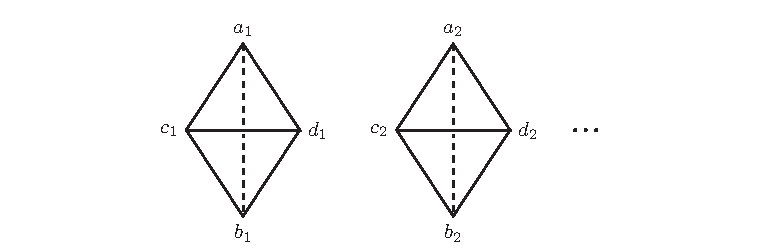
\includegraphics[width=.96\textwidth]{figures/4-14-3.pdf}\\图 4.14.3\par\medskip
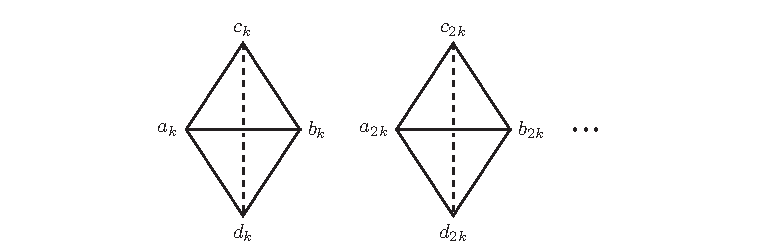
\includegraphics[width=.96\textwidth]{figures/4-14-4.pdf}\\图 4.14.4
\end{center}
\item 实 $n$ 维射影空间与复 $n$ 维射影空间有什么关系？
\item $n$ 维欧氏空间中的任一对象，在实 $n$ 维射影空间中都有一个像。解释这一点。单位球、单位立方体的像分别是什么？
\end{enumerate}
